\documentclass[12pt,letterpaper]{article}
\usepackage[letterpaper,margin=0in]{geometry}
\usepackage[T1]{fontenc}
\usepackage{lmodern}
\usepackage{tikz}
\usetikzlibrary{calc}
\pdfmapfile{+lm.map}
\pagestyle{empty}
\hyphenpenalty=10000
\exhyphenpenalty=10000
\setlength{\parindent}{0pt}
\begin{document}
\noindent\begin{tikzpicture}[remember picture,overlay,x=1in,y=1in,shift={(current page.south west)}]
\node[anchor=north west,inner sep=0pt,align=left,text width=7.18in,font=\fontsize{13}{17}\selectfont] at (0.64,10.48) {Week 20 / Averaging / K--1};
\draw[line width=.5pt] (.64,10.13)--(7.86,10.13);
\node[anchor=north west,inner sep=0pt,align=left,text width=7.18in,font=\fontsize{9.5}{13.5}\selectfont] at (0.64,0.48) {Bellingham Math Circle / Week 20 / GA20-K-v3};
\node[anchor=north east,inner sep=0pt,font=\fontsize{9.5}{12}\selectfont] at (7.86,.48) {1};
\node[anchor=north west,inner sep=0pt,align=left,text width=7.18in,font=\fontsize{12.5}{16.5}\selectfont] at (0.64,9.86) {Squares keep their stacks. A circle holds one equal share of the stacks joined to it. Make one equal pile for each joined shape, including empty shapes. Every circle must work at once. Use spare cubes to copy and share.};
\node[anchor=north west,inner sep=0pt,align=left,text width=7.18in,font=\fontsize{16}{20}\selectfont] at (0.64,6.65) {\textbf{Problem 1:} Make the circle stacks on all four boards.};
\node[anchor=north west,inner sep=0pt,align=left,text width=7.18in,font=\fontsize{12.5}{16.5}\selectfont] at (0.64,8.88) {Example};
\node[anchor=north west,inner sep=0pt,align=left,text width=1.5in,font=\fontsize{11}{15}\selectfont] at (0.74,8.56) {Before};
\node[anchor=north west,inner sep=0pt,align=left,text width=2.95in,font=\fontsize{11}{15}\selectfont] at (2.93,8.56) {Copy; share on both mats};
\node[anchor=north west,inner sep=0pt,align=left,text width=1.5in,font=\fontsize{11}{15}\selectfont] at (6.36,8.56) {After};
\node[draw,fill=white,rectangle,line width=.8pt,minimum size=0.62in,inner sep=0pt] (beforezero) at (1.1,8.02) {};
\node[font=\fontsize{14}{16}\selectfont] at (1.1,8.17) {0};
\node[draw,fill=white,rectangle,line width=.8pt,minimum size=0.62in,inner sep=0pt] (beforesix) at (2.0,8.02) {};
\node[font=\fontsize{14}{16}\selectfont] at (2.0,8.17) {6};
\draw[fill=black!20,line width=.45pt] (1.858,7.903) rectangle (1.932,7.976999999999999);
\draw[fill=black!20,line width=.45pt] (1.963,7.903) rectangle (2.037,7.976999999999999);
\draw[fill=black!20,line width=.45pt] (2.068,7.903) rectangle (2.142,7.976999999999999);
\draw[fill=black!20,line width=.45pt] (1.858,7.797999999999999) rectangle (1.932,7.871999999999999);
\draw[fill=black!20,line width=.45pt] (1.963,7.797999999999999) rectangle (2.037,7.871999999999999);
\draw[fill=black!20,line width=.45pt] (2.068,7.797999999999999) rectangle (2.142,7.871999999999999);
\node[draw,fill=white,circle,line width=.8pt,minimum size=0.62in,inner sep=0pt] (beforecircle) at (1.55,7.39) {};
\draw[line width=.85pt] (beforezero)--(beforecircle);
\draw[line width=.85pt] (beforesix)--(beforecircle);
\node[draw,fill=white,rectangle,line width=.8pt,minimum size=0.62in,inner sep=0pt] (afterzero) at (6.58,8.02) {};
\node[font=\fontsize{14}{16}\selectfont] at (6.58,8.17) {0};
\node[draw,fill=white,rectangle,line width=.8pt,minimum size=0.62in,inner sep=0pt] (aftersix) at (7.48,8.02) {};
\node[font=\fontsize{14}{16}\selectfont] at (7.48,8.17) {6};
\draw[fill=black!20,line width=.45pt] (7.338,7.903) rectangle (7.412,7.976999999999999);
\draw[fill=black!20,line width=.45pt] (7.4430000000000005,7.903) rectangle (7.517,7.976999999999999);
\draw[fill=black!20,line width=.45pt] (7.548000000000001,7.903) rectangle (7.622000000000001,7.976999999999999);
\draw[fill=black!20,line width=.45pt] (7.338,7.797999999999999) rectangle (7.412,7.871999999999999);
\draw[fill=black!20,line width=.45pt] (7.4430000000000005,7.797999999999999) rectangle (7.517,7.871999999999999);
\draw[fill=black!20,line width=.45pt] (7.548000000000001,7.797999999999999) rectangle (7.622000000000001,7.871999999999999);
\node[draw,fill=white,circle,line width=.8pt,minimum size=0.62in,inner sep=0pt] (aftercircle) at (7.03,7.39) {};
\node[font=\fontsize{14}{16}\selectfont] at (7.03,7.54) {3};
\draw[fill=black!20,line width=.45pt] (6.888,7.273) rectangle (6.962,7.3469999999999995);
\draw[fill=black!20,line width=.45pt] (6.993,7.273) rectangle (7.067,7.3469999999999995);
\draw[fill=black!20,line width=.45pt] (7.098000000000001,7.273) rectangle (7.172000000000001,7.3469999999999995);
\draw[line width=.85pt] (afterzero)--(aftercircle);
\draw[line width=.85pt] (aftersix)--(aftercircle);
\node[anchor=north west,inner sep=0pt,align=left,text width=0.75in,font=\fontsize{9.5}{13.5}\selectfont] at (2.92,8.15) {6 spare\\cubes};
\draw[fill=black!20,line width=.45pt] (3.088,7.493) rectangle (3.162,7.567);
\draw[fill=black!20,line width=.45pt] (3.193,7.493) rectangle (3.267,7.567);
\draw[fill=black!20,line width=.45pt] (3.298,7.493) rectangle (3.372,7.567);
\draw[fill=black!20,line width=.45pt] (3.088,7.388) rectangle (3.162,7.462);
\draw[fill=black!20,line width=.45pt] (3.193,7.388) rectangle (3.267,7.462);
\draw[fill=black!20,line width=.45pt] (3.298,7.388) rectangle (3.372,7.462);
\draw[->,line width=.8pt] (3.66,7.76)--(3.99,7.76);
\node[anchor=north west,inner sep=0pt,align=left,text width=0.8in,font=\fontsize{9.5}{13.5}\selectfont] at (4.13,8.2) {0's mat};
\node[anchor=north west,inner sep=0pt,align=left,text width=0.8in,font=\fontsize{9.5}{13.5}\selectfont] at (5.1,8.2) {6's mat};
\draw[dashed,rounded corners=.04in,line width=.6pt] (4.140000000000001,7.45) rectangle (4.84,8.05);
\draw[fill=black!20,line width=.45pt] (4.348,7.768) rectangle (4.422,7.842);
\draw[fill=black!20,line width=.45pt] (4.453,7.768) rectangle (4.527,7.842);
\draw[fill=black!20,line width=.45pt] (4.558000000000001,7.768) rectangle (4.632000000000001,7.842);
\draw[dashed,rounded corners=.04in,line width=.6pt] (5.11,7.45) rectangle (5.81,8.05);
\draw[fill=black!20,line width=.45pt] (5.318,7.768) rectangle (5.3919999999999995,7.842);
\draw[fill=black!20,line width=.45pt] (5.423,7.768) rectangle (5.497,7.842);
\draw[fill=black!20,line width=.45pt] (5.5280000000000005,7.768) rectangle (5.602,7.842);
\node[anchor=north west,inner sep=0pt,align=left,text width=1.8in,font=\fontsize{10.5}{14.5}\selectfont] at (4.27,7.34) {3 each};
\node[anchor=north west,inner sep=0pt,align=left,text width=7.18in,font=\fontsize{11}{15}\selectfont] at (0.64,6.99) {Both square stacks stay. Use two mats, even for 0.};
\node[draw,fill=white,rectangle,line width=1.05pt,minimum size=1.19in,inner sep=0pt,font=\fontsize{23}{25}\selectfont] (g1a) at (1.53,5.6499999999999995) {};
\node[font=\fontsize{23}{26}\selectfont] at (1.53,5.85) {0};
\node[draw,fill=white,rectangle,line width=1.05pt,minimum size=1.19in,inner sep=0pt,font=\fontsize{23}{25}\selectfont] (g1b) at (2.9699999999999998,5.6499999999999995) {};
\node[font=\fontsize{23}{26}\selectfont] at (2.9699999999999998,5.85) {2};
\fill (2.88,5.499999999999999) circle[radius=.038in];
\fill (3.0599999999999996,5.499999999999999) circle[radius=.038in];
\node[draw,fill=white,circle,line width=1.05pt,minimum size=1.19in,inner sep=0pt,font=\fontsize{23}{25}\selectfont] (g1c) at (2.25,4.35) {};
\draw[line width=1.15pt] (g1a)--(g1c);
\draw[line width=1.15pt] (g1b)--(g1c);
\node[draw,fill=white,rectangle,line width=1.05pt,minimum size=1.19in,inner sep=0pt,font=\fontsize{23}{25}\selectfont] (g2a) at (5.53,5.6499999999999995) {};
\node[font=\fontsize{23}{26}\selectfont] at (5.53,5.85) {2};
\fill (5.44,5.499999999999999) circle[radius=.038in];
\fill (5.62,5.499999999999999) circle[radius=.038in];
\node[draw,fill=white,rectangle,line width=1.05pt,minimum size=1.19in,inner sep=0pt,font=\fontsize{23}{25}\selectfont] (g2b) at (6.97,5.6499999999999995) {};
\node[font=\fontsize{23}{26}\selectfont] at (6.97,5.85) {4};
\fill (6.79,5.499999999999999) circle[radius=.038in];
\fill (6.97,5.499999999999999) circle[radius=.038in];
\fill (7.1499999999999995,5.499999999999999) circle[radius=.038in];
\fill (6.79,5.34) circle[radius=.038in];
\node[draw,fill=white,circle,line width=1.05pt,minimum size=1.19in,inner sep=0pt,font=\fontsize{23}{25}\selectfont] (g2c) at (6.25,4.35) {};
\draw[line width=1.15pt] (g2a)--(g2c);
\draw[line width=1.15pt] (g2b)--(g2c);
\node[draw,fill=white,rectangle,line width=1.05pt,minimum size=1.19in,inner sep=0pt,font=\fontsize{23}{25}\selectfont] (g3a) at (1.53,2.9699999999999998) {};
\node[font=\fontsize{23}{26}\selectfont] at (1.53,3.17) {0};
\node[draw,fill=white,rectangle,line width=1.05pt,minimum size=1.19in,inner sep=0pt,font=\fontsize{23}{25}\selectfont] (g3b) at (2.9699999999999998,2.9699999999999998) {};
\node[font=\fontsize{23}{26}\selectfont] at (2.9699999999999998,3.17) {4};
\fill (2.7899999999999996,2.82) circle[radius=.038in];
\fill (2.9699999999999998,2.82) circle[radius=.038in];
\fill (3.15,2.82) circle[radius=.038in];
\fill (2.7899999999999996,2.6599999999999997) circle[radius=.038in];
\node[draw,fill=white,circle,line width=1.05pt,minimum size=1.19in,inner sep=0pt,font=\fontsize{23}{25}\selectfont] (g3c) at (2.25,1.67) {};
\draw[line width=1.15pt] (g3a)--(g3c);
\draw[line width=1.15pt] (g3b)--(g3c);
\node[draw,fill=white,rectangle,line width=1.05pt,minimum size=1.19in,inner sep=0pt,font=\fontsize{23}{25}\selectfont] (g4a) at (5.53,2.9699999999999998) {};
\node[font=\fontsize{23}{26}\selectfont] at (5.53,3.17) {2};
\fill (5.44,2.82) circle[radius=.038in];
\fill (5.62,2.82) circle[radius=.038in];
\node[draw,fill=white,rectangle,line width=1.05pt,minimum size=1.19in,inner sep=0pt,font=\fontsize{23}{25}\selectfont] (g4b) at (6.97,2.9699999999999998) {};
\node[font=\fontsize{23}{26}\selectfont] at (6.97,3.17) {6};
\fill (6.79,2.82) circle[radius=.038in];
\fill (6.97,2.82) circle[radius=.038in];
\fill (7.1499999999999995,2.82) circle[radius=.038in];
\fill (6.79,2.6599999999999997) circle[radius=.038in];
\fill (6.97,2.6599999999999997) circle[radius=.038in];
\fill (7.1499999999999995,2.6599999999999997) circle[radius=.038in];
\node[draw,fill=white,circle,line width=1.05pt,minimum size=1.19in,inner sep=0pt,font=\fontsize{23}{25}\selectfont] (g4c) at (6.25,1.67) {};
\draw[line width=1.15pt] (g4a)--(g4c);
\draw[line width=1.15pt] (g4b)--(g4c);
\end{tikzpicture}\newpage
\noindent
\begin{tikzpicture}[remember picture,overlay,x=1in,y=1in,shift={(current page.south west)}]
\node[anchor=north west,inner sep=0pt,align=left,text width=7.18in,font=\fontsize{13}{17}\selectfont] at (0.64,10.48) {Week 20 / Averaging / K--1};
\draw[line width=.5pt] (.64,10.13)--(7.86,10.13);
\node[anchor=north west,inner sep=0pt,align=left,text width=7.18in,font=\fontsize{9.5}{13.5}\selectfont] at (0.64,0.48) {Bellingham Math Circle / Week 20 / GA20-K-v3};
\node[anchor=north east,inner sep=0pt,font=\fontsize{9.5}{12}\selectfont] at (7.86,.48) {2};
\node[anchor=north west,inner sep=0pt,align=left,text width=7.18in,font=\fontsize{16}{20}\selectfont] at (0.64,7.3) {\textbf{Problem 2:} Make all the circle stacks. Both circles on a board must work at the same time.};
\node[anchor=north west,inner sep=0pt,align=left,text width=7.18in,font=\fontsize{12.5}{16.5}\selectfont] at (0.64,9.86) {Example: both circles work.};
\node[draw,fill=white,rectangle,line width=.8pt,minimum size=0.68in,inner sep=0pt] (chain0) at (1.4,9.1) {};
\node[font=\fontsize{14}{16}\selectfont] at (1.4,9.25) {2};
\draw[fill=black!20,line width=.45pt] (1.3105,8.982999999999999) rectangle (1.3844999999999998,9.057);
\draw[fill=black!20,line width=.45pt] (1.4155,8.982999999999999) rectangle (1.4894999999999998,9.057);
\node[draw,fill=white,circle,line width=.8pt,minimum size=0.68in,inner sep=0pt] (chain1) at (3.3,9.1) {};
\node[font=\fontsize{14}{16}\selectfont] at (3.3,9.25) {3};
\draw[fill=black!20,line width=.45pt] (3.158,8.982999999999999) rectangle (3.2319999999999998,9.057);
\draw[fill=black!20,line width=.45pt] (3.263,8.982999999999999) rectangle (3.3369999999999997,9.057);
\draw[fill=black!20,line width=.45pt] (3.368,8.982999999999999) rectangle (3.4419999999999997,9.057);
\node[draw,fill=white,circle,line width=.8pt,minimum size=0.68in,inner sep=0pt] (chain2) at (5.199999999999999,9.1) {};
\node[font=\fontsize{14}{16}\selectfont] at (5.199999999999999,9.25) {4};
\draw[fill=black!20,line width=.45pt] (5.057999999999999,8.982999999999999) rectangle (5.131999999999999,9.057);
\draw[fill=black!20,line width=.45pt] (5.162999999999999,8.982999999999999) rectangle (5.236999999999999,9.057);
\draw[fill=black!20,line width=.45pt] (5.268,8.982999999999999) rectangle (5.342,9.057);
\draw[fill=black!20,line width=.45pt] (5.057999999999999,8.877999999999998) rectangle (5.131999999999999,8.952);
\node[draw,fill=white,rectangle,line width=.8pt,minimum size=0.68in,inner sep=0pt] (chain3) at (7.1,9.1) {};
\node[font=\fontsize{14}{16}\selectfont] at (7.1,9.25) {5};
\draw[fill=black!20,line width=.45pt] (6.957999999999999,8.982999999999999) rectangle (7.031999999999999,9.057);
\draw[fill=black!20,line width=.45pt] (7.063,8.982999999999999) rectangle (7.137,9.057);
\draw[fill=black!20,line width=.45pt] (7.168,8.982999999999999) rectangle (7.242,9.057);
\draw[fill=black!20,line width=.45pt] (6.957999999999999,8.877999999999998) rectangle (7.031999999999999,8.952);
\draw[fill=black!20,line width=.45pt] (7.063,8.877999999999998) rectangle (7.137,8.952);
\draw[line width=.85pt] (chain0)--(chain1);
\draw[line width=.85pt] (chain1)--(chain2);
\draw[line width=.85pt] (chain2)--(chain3);
\node[anchor=north west,inner sep=0pt,align=left,text width=1.45in,font=\fontsize{10.5}{14.5}\selectfont] at (0.64,8.62) {Check 3};
\node[anchor=north west,inner sep=0pt,align=left,text width=1.5in,font=\fontsize{10.5}{14.5}\selectfont] at (2.39,8.62) {Share copies};
\node[draw,fill=white,rectangle,line width=.8pt,minimum size=0.55in,inner sep=0pt] (copy30) at (0.94,8.17) {};
\node[font=\fontsize{14}{16}\selectfont] at (0.94,8.32) {2};
\draw[fill=black!20,line width=.45pt] (0.8504999999999999,8.052999999999999) rectangle (0.9245,8.127);
\draw[fill=black!20,line width=.45pt] (0.9554999999999999,8.052999999999999) rectangle (1.0294999999999999,8.127);
\node[draw,fill=white,circle,line width=.8pt,minimum size=0.55in,inner sep=0pt] (copy31) at (1.5899999999999999,8.17) {};
\node[font=\fontsize{14}{16}\selectfont] at (1.5899999999999999,8.32) {4};
\draw[fill=black!20,line width=.45pt] (1.448,8.052999999999999) rectangle (1.5219999999999998,8.127);
\draw[fill=black!20,line width=.45pt] (1.553,8.052999999999999) rectangle (1.6269999999999998,8.127);
\draw[fill=black!20,line width=.45pt] (1.658,8.052999999999999) rectangle (1.7319999999999998,8.127);
\draw[fill=black!20,line width=.45pt] (1.448,7.9479999999999995) rectangle (1.5219999999999998,8.022);
\draw[->,line width=.8pt] (1.9300000000000002,8.17)--(2.22,8.17);
\draw[dashed,rounded corners=.04in,line width=.6pt] (2.33,7.89) rectangle (2.8899999999999997,8.45);
\draw[fill=black!20,line width=.45pt] (2.468,8.187999999999999) rectangle (2.542,8.262);
\draw[fill=black!20,line width=.45pt] (2.573,8.187999999999999) rectangle (2.647,8.262);
\draw[fill=black!20,line width=.45pt] (2.678,8.187999999999999) rectangle (2.752,8.262);
\draw[dashed,rounded corners=.04in,line width=.6pt] (3.0200000000000005,7.89) rectangle (3.58,8.45);
\draw[fill=black!20,line width=.45pt] (3.1580000000000004,8.187999999999999) rectangle (3.232,8.262);
\draw[fill=black!20,line width=.45pt] (3.2630000000000003,8.187999999999999) rectangle (3.337,8.262);
\draw[fill=black!20,line width=.45pt] (3.3680000000000003,8.187999999999999) rectangle (3.442,8.262);
\node[anchor=north west,inner sep=0pt,align=left,text width=1.55in,font=\fontsize{10.5}{14.5}\selectfont] at (2.39,7.83) {3 each};
\node[anchor=north west,inner sep=0pt,align=left,text width=1.45in,font=\fontsize{10.5}{14.5}\selectfont] at (4.44,8.62) {Check 4};
\node[anchor=north west,inner sep=0pt,align=left,text width=1.5in,font=\fontsize{10.5}{14.5}\selectfont] at (6.19,8.62) {Share copies};
\node[draw,fill=white,circle,line width=.8pt,minimum size=0.55in,inner sep=0pt] (copy40) at (4.74,8.17) {};
\node[font=\fontsize{14}{16}\selectfont] at (4.74,8.32) {3};
\draw[fill=black!20,line width=.45pt] (4.598,8.052999999999999) rectangle (4.672,8.127);
\draw[fill=black!20,line width=.45pt] (4.703,8.052999999999999) rectangle (4.777,8.127);
\draw[fill=black!20,line width=.45pt] (4.808000000000001,8.052999999999999) rectangle (4.882000000000001,8.127);
\node[draw,fill=white,rectangle,line width=.8pt,minimum size=0.55in,inner sep=0pt] (copy41) at (5.390000000000001,8.17) {};
\node[font=\fontsize{14}{16}\selectfont] at (5.390000000000001,8.32) {5};
\draw[fill=black!20,line width=.45pt] (5.248,8.052999999999999) rectangle (5.322,8.127);
\draw[fill=black!20,line width=.45pt] (5.353000000000001,8.052999999999999) rectangle (5.4270000000000005,8.127);
\draw[fill=black!20,line width=.45pt] (5.458000000000001,8.052999999999999) rectangle (5.532000000000001,8.127);
\draw[fill=black!20,line width=.45pt] (5.248,7.9479999999999995) rectangle (5.322,8.022);
\draw[fill=black!20,line width=.45pt] (5.353000000000001,7.9479999999999995) rectangle (5.4270000000000005,8.022);
\draw[->,line width=.8pt] (5.73,8.17)--(6.0200000000000005,8.17);
\draw[dashed,rounded corners=.04in,line width=.6pt] (6.13,7.89) rectangle (6.69,8.45);
\draw[fill=black!20,line width=.45pt] (6.268,8.187999999999999) rectangle (6.342,8.262);
\draw[fill=black!20,line width=.45pt] (6.373,8.187999999999999) rectangle (6.447,8.262);
\draw[fill=black!20,line width=.45pt] (6.478000000000001,8.187999999999999) rectangle (6.5520000000000005,8.262);
\draw[fill=black!20,line width=.45pt] (6.268,8.082999999999998) rectangle (6.342,8.157);
\draw[dashed,rounded corners=.04in,line width=.6pt] (6.82,7.89) rectangle (7.380000000000001,8.45);
\draw[fill=black!20,line width=.45pt] (6.958,8.187999999999999) rectangle (7.032,8.262);
\draw[fill=black!20,line width=.45pt] (7.063000000000001,8.187999999999999) rectangle (7.1370000000000005,8.262);
\draw[fill=black!20,line width=.45pt] (7.168000000000001,8.187999999999999) rectangle (7.242000000000001,8.262);
\draw[fill=black!20,line width=.45pt] (6.958,8.082999999999998) rectangle (7.032,8.157);
\node[anchor=north west,inner sep=0pt,align=left,text width=1.55in,font=\fontsize{10.5}{14.5}\selectfont] at (6.19,7.83) {4 each};
\node[anchor=north west,inner sep=0pt,align=left,text width=7.18in,font=\fontsize{10.5}{14.5}\selectfont] at (0.64,7.62) {Check both circles on the same board. Keep all four stacks.};
\node[draw,fill=white,rectangle,line width=1.05pt,minimum size=1.19in,inner sep=0pt,font=\fontsize{23}{25}\selectfont] (g50) at (1.4,6.12) {};
\node[font=\fontsize{23}{26}\selectfont] at (1.4,6.32) {0};
\node[draw,fill=white,circle,line width=1.05pt,minimum size=1.19in,inner sep=0pt,font=\fontsize{23}{25}\selectfont] (g51) at (3.3,6.12) {};
\node[draw,fill=white,circle,line width=1.05pt,minimum size=1.19in,inner sep=0pt,font=\fontsize{23}{25}\selectfont] (g52) at (5.2,6.12) {};
\node[draw,fill=white,rectangle,line width=1.05pt,minimum size=1.19in,inner sep=0pt,font=\fontsize{23}{25}\selectfont] (g53) at (7.1,6.12) {};
\node[font=\fontsize{23}{26}\selectfont] at (7.1,6.32) {3};
\fill (6.92,5.97) circle[radius=.038in];
\fill (7.1,5.97) circle[radius=.038in];
\fill (7.279999999999999,5.97) circle[radius=.038in];
\draw[line width=1.15pt] (g50)--(g51);
\draw[line width=1.15pt] (g51)--(g52);
\draw[line width=1.15pt] (g52)--(g53);
\node[draw,fill=white,rectangle,line width=1.05pt,minimum size=1.19in,inner sep=0pt,font=\fontsize{23}{25}\selectfont] (g60) at (1.4,4.6) {};
\node[font=\fontsize{23}{26}\selectfont] at (1.4,4.8) {3};
\fill (1.22,4.449999999999999) circle[radius=.038in];
\fill (1.4,4.449999999999999) circle[radius=.038in];
\fill (1.5799999999999998,4.449999999999999) circle[radius=.038in];
\node[draw,fill=white,circle,line width=1.05pt,minimum size=1.19in,inner sep=0pt,font=\fontsize{23}{25}\selectfont] (g61) at (3.3,4.6) {};
\node[draw,fill=white,circle,line width=1.05pt,minimum size=1.19in,inner sep=0pt,font=\fontsize{23}{25}\selectfont] (g62) at (5.2,4.6) {};
\node[draw,fill=white,rectangle,line width=1.05pt,minimum size=1.19in,inner sep=0pt,font=\fontsize{23}{25}\selectfont] (g63) at (7.1,4.6) {};
\node[font=\fontsize{23}{26}\selectfont] at (7.1,4.8) {0};
\draw[line width=1.15pt] (g60)--(g61);
\draw[line width=1.15pt] (g61)--(g62);
\draw[line width=1.15pt] (g62)--(g63);
\node[draw,fill=white,rectangle,line width=1.05pt,minimum size=1.19in,inner sep=0pt,font=\fontsize{23}{25}\selectfont] (g70) at (1.4,3.08) {};
\node[font=\fontsize{23}{26}\selectfont] at (1.4,3.2800000000000002) {0};
\node[draw,fill=white,circle,line width=1.05pt,minimum size=1.19in,inner sep=0pt,font=\fontsize{23}{25}\selectfont] (g71) at (3.3,3.08) {};
\node[draw,fill=white,circle,line width=1.05pt,minimum size=1.19in,inner sep=0pt,font=\fontsize{23}{25}\selectfont] (g72) at (5.2,3.08) {};
\node[draw,fill=white,rectangle,line width=1.05pt,minimum size=1.19in,inner sep=0pt,font=\fontsize{23}{25}\selectfont] (g73) at (7.1,3.08) {};
\node[font=\fontsize{23}{26}\selectfont] at (7.1,3.2800000000000002) {6};
\fill (6.92,2.93) circle[radius=.038in];
\fill (7.1,2.93) circle[radius=.038in];
\fill (7.279999999999999,2.93) circle[radius=.038in];
\fill (6.92,2.77) circle[radius=.038in];
\fill (7.1,2.77) circle[radius=.038in];
\fill (7.279999999999999,2.77) circle[radius=.038in];
\draw[line width=1.15pt] (g70)--(g71);
\draw[line width=1.15pt] (g71)--(g72);
\draw[line width=1.15pt] (g72)--(g73);
\node[draw,fill=white,rectangle,line width=1.05pt,minimum size=1.19in,inner sep=0pt,font=\fontsize{23}{25}\selectfont] (g80) at (1.4,1.56) {};
\node[font=\fontsize{23}{26}\selectfont] at (1.4,1.76) {6};
\fill (1.22,1.4100000000000001) circle[radius=.038in];
\fill (1.4,1.4100000000000001) circle[radius=.038in];
\fill (1.5799999999999998,1.4100000000000001) circle[radius=.038in];
\fill (1.22,1.25) circle[radius=.038in];
\fill (1.4,1.25) circle[radius=.038in];
\fill (1.5799999999999998,1.25) circle[radius=.038in];
\node[draw,fill=white,circle,line width=1.05pt,minimum size=1.19in,inner sep=0pt,font=\fontsize{23}{25}\selectfont] (g81) at (3.3,1.56) {};
\node[draw,fill=white,circle,line width=1.05pt,minimum size=1.19in,inner sep=0pt,font=\fontsize{23}{25}\selectfont] (g82) at (5.2,1.56) {};
\node[draw,fill=white,rectangle,line width=1.05pt,minimum size=1.19in,inner sep=0pt,font=\fontsize{23}{25}\selectfont] (g83) at (7.1,1.56) {};
\node[font=\fontsize{23}{26}\selectfont] at (7.1,1.76) {0};
\draw[line width=1.15pt] (g80)--(g81);
\draw[line width=1.15pt] (g81)--(g82);
\draw[line width=1.15pt] (g82)--(g83);
\end{tikzpicture}\newpage
\noindent\begin{tikzpicture}[remember picture,overlay,x=1in,y=1in,shift={(current page.south west)}]
\node[anchor=north west,inner sep=0pt,align=left,text width=7.18in,font=\fontsize{13}{17}\selectfont] at (0.64,10.48) {Week 20 / Averaging / K--1};
\draw[line width=.5pt] (.64,10.13)--(7.86,10.13);
\node[anchor=north west,inner sep=0pt,align=left,text width=7.18in,font=\fontsize{9.5}{13.5}\selectfont] at (0.64,0.48) {Bellingham Math Circle / Week 20 / GA20-K-v3};
\node[anchor=north east,inner sep=0pt,font=\fontsize{9.5}{12}\selectfont] at (7.86,.48) {3};
\node[anchor=north west,inner sep=0pt,align=left,text width=7.18in,font=\fontsize{16}{20}\selectfont] at (0.64,9.86) {\textbf{Problem 3:} Put 2 cubes in the circle and use 0 to 3 cubes in each square. Find every way that works.};
\node[draw,fill=white,rectangle,line width=1.05pt,minimum size=1.19in,inner sep=0pt,font=\fontsize{23}{25}\selectfont] (g9a) at (4.25,8.45) {};
\node[draw,fill=white,rectangle,line width=1.05pt,minimum size=1.19in,inner sep=0pt,font=\fontsize{23}{25}\selectfont] (g9b) at (2.9,6.2) {};
\node[draw,fill=white,rectangle,line width=1.05pt,minimum size=1.19in,inner sep=0pt,font=\fontsize{23}{25}\selectfont] (g9c) at (5.6,6.2) {};
\node[draw,fill=white,circle,line width=1.05pt,minimum size=1.19in,inner sep=0pt,font=\fontsize{23}{25}\selectfont] (g9u) at (4.25,6.95) {};
\node[font=\fontsize{23}{26}\selectfont] at (4.25,7.15) {2};
\fill (4.16,6.8) circle[radius=.038in];
\fill (4.34,6.8) circle[radius=.038in];
\draw[line width=1.15pt] (g9a)--(g9u);
\draw[line width=1.15pt] (g9b)--(g9u);
\draw[line width=1.15pt] (g9c)--(g9u);
\node[draw,fill=white,rectangle,line width=1.05pt,minimum size=0.42in,inner sep=0pt,font=\fontsize{12}{25}\selectfont] (g10a) at (1.3,4.85) {};
\node[draw,fill=white,rectangle,line width=1.05pt,minimum size=0.42in,inner sep=0pt,font=\fontsize{12}{25}\selectfont] (g10b) at (0.8500000000000001,3.9) {};
\node[draw,fill=white,rectangle,line width=1.05pt,minimum size=0.42in,inner sep=0pt,font=\fontsize{12}{25}\selectfont] (g10c) at (1.75,3.9) {};
\node[draw,fill=white,circle,line width=1.05pt,minimum size=0.42in,inner sep=0pt,font=\fontsize{12}{25}\selectfont] (g10u) at (1.3,4.25) {2};
\draw[line width=1.15pt] (g10a)--(g10u);
\draw[line width=1.15pt] (g10b)--(g10u);
\draw[line width=1.15pt] (g10c)--(g10u);
\node[draw,fill=white,rectangle,line width=1.05pt,minimum size=0.42in,inner sep=0pt,font=\fontsize{12}{25}\selectfont] (g11a) at (2.775,4.85) {};
\node[draw,fill=white,rectangle,line width=1.05pt,minimum size=0.42in,inner sep=0pt,font=\fontsize{12}{25}\selectfont] (g11b) at (2.3249999999999997,3.9) {};
\node[draw,fill=white,rectangle,line width=1.05pt,minimum size=0.42in,inner sep=0pt,font=\fontsize{12}{25}\selectfont] (g11c) at (3.225,3.9) {};
\node[draw,fill=white,circle,line width=1.05pt,minimum size=0.42in,inner sep=0pt,font=\fontsize{12}{25}\selectfont] (g11u) at (2.775,4.25) {2};
\draw[line width=1.15pt] (g11a)--(g11u);
\draw[line width=1.15pt] (g11b)--(g11u);
\draw[line width=1.15pt] (g11c)--(g11u);
\node[draw,fill=white,rectangle,line width=1.05pt,minimum size=0.42in,inner sep=0pt,font=\fontsize{12}{25}\selectfont] (g12a) at (4.25,4.85) {};
\node[draw,fill=white,rectangle,line width=1.05pt,minimum size=0.42in,inner sep=0pt,font=\fontsize{12}{25}\selectfont] (g12b) at (3.8,3.9) {};
\node[draw,fill=white,rectangle,line width=1.05pt,minimum size=0.42in,inner sep=0pt,font=\fontsize{12}{25}\selectfont] (g12c) at (4.7,3.9) {};
\node[draw,fill=white,circle,line width=1.05pt,minimum size=0.42in,inner sep=0pt,font=\fontsize{12}{25}\selectfont] (g12u) at (4.25,4.25) {2};
\draw[line width=1.15pt] (g12a)--(g12u);
\draw[line width=1.15pt] (g12b)--(g12u);
\draw[line width=1.15pt] (g12c)--(g12u);
\node[draw,fill=white,rectangle,line width=1.05pt,minimum size=0.42in,inner sep=0pt,font=\fontsize{12}{25}\selectfont] (g13a) at (5.725,4.85) {};
\node[draw,fill=white,rectangle,line width=1.05pt,minimum size=0.42in,inner sep=0pt,font=\fontsize{12}{25}\selectfont] (g13b) at (5.2749999999999995,3.9) {};
\node[draw,fill=white,rectangle,line width=1.05pt,minimum size=0.42in,inner sep=0pt,font=\fontsize{12}{25}\selectfont] (g13c) at (6.175,3.9) {};
\node[draw,fill=white,circle,line width=1.05pt,minimum size=0.42in,inner sep=0pt,font=\fontsize{12}{25}\selectfont] (g13u) at (5.725,4.25) {2};
\draw[line width=1.15pt] (g13a)--(g13u);
\draw[line width=1.15pt] (g13b)--(g13u);
\draw[line width=1.15pt] (g13c)--(g13u);
\node[draw,fill=white,rectangle,line width=1.05pt,minimum size=0.42in,inner sep=0pt,font=\fontsize{12}{25}\selectfont] (g14a) at (7.2,4.85) {};
\node[draw,fill=white,rectangle,line width=1.05pt,minimum size=0.42in,inner sep=0pt,font=\fontsize{12}{25}\selectfont] (g14b) at (6.75,3.9) {};
\node[draw,fill=white,rectangle,line width=1.05pt,minimum size=0.42in,inner sep=0pt,font=\fontsize{12}{25}\selectfont] (g14c) at (7.65,3.9) {};
\node[draw,fill=white,circle,line width=1.05pt,minimum size=0.42in,inner sep=0pt,font=\fontsize{12}{25}\selectfont] (g14u) at (7.2,4.25) {2};
\draw[line width=1.15pt] (g14a)--(g14u);
\draw[line width=1.15pt] (g14b)--(g14u);
\draw[line width=1.15pt] (g14c)--(g14u);
\node[draw,fill=white,rectangle,line width=1.05pt,minimum size=0.42in,inner sep=0pt,font=\fontsize{12}{25}\selectfont] (g15a) at (1.3,3.0500000000000003) {};
\node[draw,fill=white,rectangle,line width=1.05pt,minimum size=0.42in,inner sep=0pt,font=\fontsize{12}{25}\selectfont] (g15b) at (0.8500000000000001,2.1) {};
\node[draw,fill=white,rectangle,line width=1.05pt,minimum size=0.42in,inner sep=0pt,font=\fontsize{12}{25}\selectfont] (g15c) at (1.75,2.1) {};
\node[draw,fill=white,circle,line width=1.05pt,minimum size=0.42in,inner sep=0pt,font=\fontsize{12}{25}\selectfont] (g15u) at (1.3,2.45) {2};
\draw[line width=1.15pt] (g15a)--(g15u);
\draw[line width=1.15pt] (g15b)--(g15u);
\draw[line width=1.15pt] (g15c)--(g15u);
\node[draw,fill=white,rectangle,line width=1.05pt,minimum size=0.42in,inner sep=0pt,font=\fontsize{12}{25}\selectfont] (g16a) at (2.775,3.0500000000000003) {};
\node[draw,fill=white,rectangle,line width=1.05pt,minimum size=0.42in,inner sep=0pt,font=\fontsize{12}{25}\selectfont] (g16b) at (2.3249999999999997,2.1) {};
\node[draw,fill=white,rectangle,line width=1.05pt,minimum size=0.42in,inner sep=0pt,font=\fontsize{12}{25}\selectfont] (g16c) at (3.225,2.1) {};
\node[draw,fill=white,circle,line width=1.05pt,minimum size=0.42in,inner sep=0pt,font=\fontsize{12}{25}\selectfont] (g16u) at (2.775,2.45) {2};
\draw[line width=1.15pt] (g16a)--(g16u);
\draw[line width=1.15pt] (g16b)--(g16u);
\draw[line width=1.15pt] (g16c)--(g16u);
\node[draw,fill=white,rectangle,line width=1.05pt,minimum size=0.42in,inner sep=0pt,font=\fontsize{12}{25}\selectfont] (g17a) at (4.25,3.0500000000000003) {};
\node[draw,fill=white,rectangle,line width=1.05pt,minimum size=0.42in,inner sep=0pt,font=\fontsize{12}{25}\selectfont] (g17b) at (3.8,2.1) {};
\node[draw,fill=white,rectangle,line width=1.05pt,minimum size=0.42in,inner sep=0pt,font=\fontsize{12}{25}\selectfont] (g17c) at (4.7,2.1) {};
\node[draw,fill=white,circle,line width=1.05pt,minimum size=0.42in,inner sep=0pt,font=\fontsize{12}{25}\selectfont] (g17u) at (4.25,2.45) {2};
\draw[line width=1.15pt] (g17a)--(g17u);
\draw[line width=1.15pt] (g17b)--(g17u);
\draw[line width=1.15pt] (g17c)--(g17u);
\node[draw,fill=white,rectangle,line width=1.05pt,minimum size=0.42in,inner sep=0pt,font=\fontsize{12}{25}\selectfont] (g18a) at (5.725,3.0500000000000003) {};
\node[draw,fill=white,rectangle,line width=1.05pt,minimum size=0.42in,inner sep=0pt,font=\fontsize{12}{25}\selectfont] (g18b) at (5.2749999999999995,2.1) {};
\node[draw,fill=white,rectangle,line width=1.05pt,minimum size=0.42in,inner sep=0pt,font=\fontsize{12}{25}\selectfont] (g18c) at (6.175,2.1) {};
\node[draw,fill=white,circle,line width=1.05pt,minimum size=0.42in,inner sep=0pt,font=\fontsize{12}{25}\selectfont] (g18u) at (5.725,2.45) {2};
\draw[line width=1.15pt] (g18a)--(g18u);
\draw[line width=1.15pt] (g18b)--(g18u);
\draw[line width=1.15pt] (g18c)--(g18u);
\node[draw,fill=white,rectangle,line width=1.05pt,minimum size=0.42in,inner sep=0pt,font=\fontsize{12}{25}\selectfont] (g19a) at (7.2,3.0500000000000003) {};
\node[draw,fill=white,rectangle,line width=1.05pt,minimum size=0.42in,inner sep=0pt,font=\fontsize{12}{25}\selectfont] (g19b) at (6.75,2.1) {};
\node[draw,fill=white,rectangle,line width=1.05pt,minimum size=0.42in,inner sep=0pt,font=\fontsize{12}{25}\selectfont] (g19c) at (7.65,2.1) {};
\node[draw,fill=white,circle,line width=1.05pt,minimum size=0.42in,inner sep=0pt,font=\fontsize{12}{25}\selectfont] (g19u) at (7.2,2.45) {2};
\draw[line width=1.15pt] (g19a)--(g19u);
\draw[line width=1.15pt] (g19b)--(g19u);
\draw[line width=1.15pt] (g19c)--(g19u);
\end{tikzpicture}\newpage
\noindent\begin{tikzpicture}[remember picture,overlay,x=1in,y=1in,shift={(current page.south west)}]
\node[anchor=north west,inner sep=0pt,align=left,text width=7.18in,font=\fontsize{13}{17}\selectfont] at (0.64,10.48) {Week 20 / Averaging / K--1};
\draw[line width=.5pt] (.64,10.13)--(7.86,10.13);
\node[anchor=north west,inner sep=0pt,align=left,text width=7.18in,font=\fontsize{9.5}{13.5}\selectfont] at (0.64,0.48) {Bellingham Math Circle / Week 20 / GA20-K-v3};
\node[anchor=north east,inner sep=0pt,font=\fontsize{9.5}{12}\selectfont] at (7.86,.48) {4};
\node[anchor=north west,inner sep=0pt,align=left,text width=7.18in,font=\fontsize{16}{20}\selectfont] at (0.64,9.86) {\textbf{Problem 4:} Use three different cards to fill the squares and circle. Find every way that works.};
\node[draw,minimum width=.65in,minimum height=.85in,font=\fontsize{23}{26}\selectfont] at (2.05,8.15) {0};
\node[draw,minimum width=.65in,minimum height=.85in,font=\fontsize{23}{26}\selectfont] at (3.15,8.15) {1};
\node[draw,minimum width=.65in,minimum height=.85in,font=\fontsize{23}{26}\selectfont] at (4.25,8.15) {2};
\node[draw,minimum width=.65in,minimum height=.85in,font=\fontsize{23}{26}\selectfont] at (5.35,8.15) {3};
\node[draw,minimum width=.65in,minimum height=.85in,font=\fontsize{23}{26}\selectfont] at (6.45,8.15) {4};
\node[draw,fill=white,rectangle,line width=1.05pt,minimum size=1.19in,inner sep=0pt,font=\fontsize{23}{25}\selectfont] (g20a) at (2.05,6.05) {};
\node[draw,fill=white,circle,line width=1.05pt,minimum size=1.19in,inner sep=0pt,font=\fontsize{23}{25}\selectfont] (g20u) at (4.25,6.05) {};
\node[draw,fill=white,rectangle,line width=1.05pt,minimum size=1.19in,inner sep=0pt,font=\fontsize{23}{25}\selectfont] (g20b) at (6.45,6.05) {};
\draw[line width=1.15pt] (g20a)--(g20u);
\draw[line width=1.15pt] (g20u)--(g20b);
\node[draw,fill=white,rectangle,line width=1.05pt,minimum size=0.48in,inner sep=0pt,font=\fontsize{12}{25}\selectfont] (g21a) at (1.27,4.6) {};
\node[draw,fill=white,circle,line width=1.05pt,minimum size=0.48in,inner sep=0pt,font=\fontsize{12}{25}\selectfont] (g21u) at (2.15,4.6) {};
\node[draw,fill=white,rectangle,line width=1.05pt,minimum size=0.48in,inner sep=0pt,font=\fontsize{12}{25}\selectfont] (g21b) at (3.03,4.6) {};
\draw[line width=1.15pt] (g21a)--(g21u);
\draw[line width=1.15pt] (g21u)--(g21b);
\node[draw,fill=white,rectangle,line width=1.05pt,minimum size=0.48in,inner sep=0pt,font=\fontsize{12}{25}\selectfont] (g22a) at (5.47,4.6) {};
\node[draw,fill=white,circle,line width=1.05pt,minimum size=0.48in,inner sep=0pt,font=\fontsize{12}{25}\selectfont] (g22u) at (6.35,4.6) {};
\node[draw,fill=white,rectangle,line width=1.05pt,minimum size=0.48in,inner sep=0pt,font=\fontsize{12}{25}\selectfont] (g22b) at (7.2299999999999995,4.6) {};
\draw[line width=1.15pt] (g22a)--(g22u);
\draw[line width=1.15pt] (g22u)--(g22b);
\node[draw,fill=white,rectangle,line width=1.05pt,minimum size=0.48in,inner sep=0pt,font=\fontsize{12}{25}\selectfont] (g23a) at (1.27,3.5) {};
\node[draw,fill=white,circle,line width=1.05pt,minimum size=0.48in,inner sep=0pt,font=\fontsize{12}{25}\selectfont] (g23u) at (2.15,3.5) {};
\node[draw,fill=white,rectangle,line width=1.05pt,minimum size=0.48in,inner sep=0pt,font=\fontsize{12}{25}\selectfont] (g23b) at (3.03,3.5) {};
\draw[line width=1.15pt] (g23a)--(g23u);
\draw[line width=1.15pt] (g23u)--(g23b);
\node[draw,fill=white,rectangle,line width=1.05pt,minimum size=0.48in,inner sep=0pt,font=\fontsize{12}{25}\selectfont] (g24a) at (5.47,3.5) {};
\node[draw,fill=white,circle,line width=1.05pt,minimum size=0.48in,inner sep=0pt,font=\fontsize{12}{25}\selectfont] (g24u) at (6.35,3.5) {};
\node[draw,fill=white,rectangle,line width=1.05pt,minimum size=0.48in,inner sep=0pt,font=\fontsize{12}{25}\selectfont] (g24b) at (7.2299999999999995,3.5) {};
\draw[line width=1.15pt] (g24a)--(g24u);
\draw[line width=1.15pt] (g24u)--(g24b);
\node[draw,fill=white,rectangle,line width=1.05pt,minimum size=0.48in,inner sep=0pt,font=\fontsize{12}{25}\selectfont] (g25a) at (1.27,2.4) {};
\node[draw,fill=white,circle,line width=1.05pt,minimum size=0.48in,inner sep=0pt,font=\fontsize{12}{25}\selectfont] (g25u) at (2.15,2.4) {};
\node[draw,fill=white,rectangle,line width=1.05pt,minimum size=0.48in,inner sep=0pt,font=\fontsize{12}{25}\selectfont] (g25b) at (3.03,2.4) {};
\draw[line width=1.15pt] (g25a)--(g25u);
\draw[line width=1.15pt] (g25u)--(g25b);
\node[draw,fill=white,rectangle,line width=1.05pt,minimum size=0.48in,inner sep=0pt,font=\fontsize{12}{25}\selectfont] (g26a) at (5.47,2.4) {};
\node[draw,fill=white,circle,line width=1.05pt,minimum size=0.48in,inner sep=0pt,font=\fontsize{12}{25}\selectfont] (g26u) at (6.35,2.4) {};
\node[draw,fill=white,rectangle,line width=1.05pt,minimum size=0.48in,inner sep=0pt,font=\fontsize{12}{25}\selectfont] (g26b) at (7.2299999999999995,2.4) {};
\draw[line width=1.15pt] (g26a)--(g26u);
\draw[line width=1.15pt] (g26u)--(g26b);
\node[draw,fill=white,rectangle,line width=1.05pt,minimum size=0.48in,inner sep=0pt,font=\fontsize{12}{25}\selectfont] (g27a) at (1.27,1.3) {};
\node[draw,fill=white,circle,line width=1.05pt,minimum size=0.48in,inner sep=0pt,font=\fontsize{12}{25}\selectfont] (g27u) at (2.15,1.3) {};
\node[draw,fill=white,rectangle,line width=1.05pt,minimum size=0.48in,inner sep=0pt,font=\fontsize{12}{25}\selectfont] (g27b) at (3.03,1.3) {};
\draw[line width=1.15pt] (g27a)--(g27u);
\draw[line width=1.15pt] (g27u)--(g27b);
\node[draw,fill=white,rectangle,line width=1.05pt,minimum size=0.48in,inner sep=0pt,font=\fontsize{12}{25}\selectfont] (g28a) at (5.47,1.3) {};
\node[draw,fill=white,circle,line width=1.05pt,minimum size=0.48in,inner sep=0pt,font=\fontsize{12}{25}\selectfont] (g28u) at (6.35,1.3) {};
\node[draw,fill=white,rectangle,line width=1.05pt,minimum size=0.48in,inner sep=0pt,font=\fontsize{12}{25}\selectfont] (g28b) at (7.2299999999999995,1.3) {};
\draw[line width=1.15pt] (g28a)--(g28u);
\draw[line width=1.15pt] (g28u)--(g28b);
\end{tikzpicture}\newpage
\noindent\begin{tikzpicture}[remember picture,overlay,x=1in,y=1in,shift={(current page.south west)}]
\node[anchor=north west,inner sep=0pt,align=left,text width=7.18in,font=\fontsize{13}{17}\selectfont] at (0.64,10.48) {Week 20 / Averaging / K--1};
\draw[line width=.5pt] (.64,10.13)--(7.86,10.13);
\node[anchor=north west,inner sep=0pt,align=left,text width=7.18in,font=\fontsize{9.5}{13.5}\selectfont] at (0.64,0.48) {Bellingham Math Circle / Week 20 / GA20-K-v3};
\node[anchor=north east,inner sep=0pt,font=\fontsize{9.5}{12}\selectfont] at (7.86,.48) {5};
\node[anchor=north west,inner sep=0pt,align=left,text width=7.18in,font=\fontsize{16}{20}\selectfont] at (0.64,9.86) {\textbf{Problem 5:} Can you make a 5-cube circle on either board while every circle works? Show why it can or cannot be done.};
\node[draw,fill=white,rectangle,line width=1.05pt,minimum size=1.19in,inner sep=0pt,font=\fontsize{23}{25}\selectfont] (g290) at (1.4,7.65) {};
\node[font=\fontsize{23}{26}\selectfont] at (1.4,7.8500000000000005) {0};
\node[draw,fill=white,circle,line width=1.05pt,minimum size=1.19in,inner sep=0pt,font=\fontsize{23}{25}\selectfont] (g291) at (3.3,7.65) {};
\node[draw,fill=white,circle,line width=1.05pt,minimum size=1.19in,inner sep=0pt,font=\fontsize{23}{25}\selectfont] (g292) at (5.2,7.65) {};
\node[draw,fill=white,rectangle,line width=1.05pt,minimum size=1.19in,inner sep=0pt,font=\fontsize{23}{25}\selectfont] (g293) at (7.1,7.65) {};
\node[font=\fontsize{23}{26}\selectfont] at (7.1,7.8500000000000005) {3};
\fill (6.92,7.5) circle[radius=.038in];
\fill (7.1,7.5) circle[radius=.038in];
\fill (7.279999999999999,7.5) circle[radius=.038in];
\draw[line width=1.15pt] (g290)--(g291);
\draw[line width=1.15pt] (g291)--(g292);
\draw[line width=1.15pt] (g292)--(g293);
\node[draw,fill=white,rectangle,line width=1.05pt,minimum size=1.19in,inner sep=0pt,font=\fontsize{23}{25}\selectfont] (g300) at (1.4,4.25) {};
\node[font=\fontsize{23}{26}\selectfont] at (1.4,4.45) {1};
\fill (1.4,4.1) circle[radius=.038in];
\node[draw,fill=white,circle,line width=1.05pt,minimum size=1.19in,inner sep=0pt,font=\fontsize{23}{25}\selectfont] (g301) at (3.3,4.25) {};
\node[draw,fill=white,circle,line width=1.05pt,minimum size=1.19in,inner sep=0pt,font=\fontsize{23}{25}\selectfont] (g302) at (5.2,4.25) {};
\node[draw,fill=white,rectangle,line width=1.05pt,minimum size=1.19in,inner sep=0pt,font=\fontsize{23}{25}\selectfont] (g303) at (7.1,4.25) {};
\node[font=\fontsize{23}{26}\selectfont] at (7.1,4.45) {4};
\fill (6.92,4.1) circle[radius=.038in];
\fill (7.1,4.1) circle[radius=.038in];
\fill (7.279999999999999,4.1) circle[radius=.038in];
\fill (6.92,3.94) circle[radius=.038in];
\draw[line width=1.15pt] (g300)--(g301);
\draw[line width=1.15pt] (g301)--(g302);
\draw[line width=1.15pt] (g302)--(g303);
\end{tikzpicture}\newpage
\noindent\begin{tikzpicture}[remember picture,overlay,x=1in,y=1in,shift={(current page.south west)}]
\node[anchor=north west,inner sep=0pt,align=left,text width=7.18in,font=\fontsize{13}{17}\selectfont] at (0.64,10.48) {Week 20 / Averaging / K--1};
\draw[line width=.5pt] (.64,10.13)--(7.86,10.13);
\node[anchor=north west,inner sep=0pt,align=left,text width=7.18in,font=\fontsize{9.5}{13.5}\selectfont] at (0.64,0.48) {Bellingham Math Circle / Week 20 / GA20-K-v3};
\node[anchor=north east,inner sep=0pt,font=\fontsize{9.5}{12}\selectfont] at (7.86,.48) {6};
\node[anchor=north west,inner sep=0pt,align=left,text width=7.18in,font=\fontsize{16}{20}\selectfont] at (0.64,9.86) {\textbf{Problem 6:} Fill the circles. Can any circle have a different number of cubes from its square?};
\node[draw,fill=white,rectangle,line width=1.05pt,minimum size=1.19in,inner sep=0pt,font=\fontsize{23}{25}\selectfont] (g31a) at (4.25,8.1) {};
\node[font=\fontsize{23}{26}\selectfont] at (4.25,8.299999999999999) {2};
\fill (4.16,7.949999999999999) circle[radius=.038in];
\fill (4.34,7.949999999999999) circle[radius=.038in];
\node[draw,fill=white,circle,line width=1.05pt,minimum size=1.19in,inner sep=0pt,font=\fontsize{23}{25}\selectfont] (g31u) at (2.9,6.3) {};
\node[draw,fill=white,circle,line width=1.05pt,minimum size=1.19in,inner sep=0pt,font=\fontsize{23}{25}\selectfont] (g31v) at (5.6,6.3) {};
\draw[line width=1.15pt] (g31a)--(g31u);
\draw[line width=1.15pt] (g31a)--(g31v);
\draw[line width=1.15pt] (g31u)--(g31v);
\node[draw,fill=white,rectangle,line width=1.05pt,minimum size=1.19in,inner sep=0pt,font=\fontsize{23}{25}\selectfont] (g32a) at (2.95,4.1) {};
\node[font=\fontsize{23}{26}\selectfont] at (2.95,4.3) {3};
\fill (2.77,3.9499999999999997) circle[radius=.038in];
\fill (2.95,3.9499999999999997) circle[radius=.038in];
\fill (3.1300000000000003,3.9499999999999997) circle[radius=.038in];
\node[draw,fill=white,circle,line width=1.05pt,minimum size=1.19in,inner sep=0pt,font=\fontsize{23}{25}\selectfont] (g32u) at (5.55,4.1) {};
\node[draw,fill=white,circle,line width=1.05pt,minimum size=1.19in,inner sep=0pt,font=\fontsize{23}{25}\selectfont] (g32v) at (5.55,1.9) {};
\node[draw,fill=white,circle,line width=1.05pt,minimum size=1.19in,inner sep=0pt,font=\fontsize{23}{25}\selectfont] (g32w) at (2.95,1.9) {};
\draw[line width=1.15pt] (g32a)--(g32u);
\draw[line width=1.15pt] (g32u)--(g32v);
\draw[line width=1.15pt] (g32v)--(g32w);
\draw[line width=1.15pt] (g32w)--(g32a);
\end{tikzpicture}\newpage
\noindent
\begin{tikzpicture}[remember picture,overlay,x=1in,y=1in,shift={(current page.south west)}]
\node[anchor=north west,inner sep=0pt,align=left,text width=7.18in,font=\fontsize{13}{17}\selectfont] at (0.64,10.48) {Week 20 / Averaging / K--1};
\draw[line width=.5pt] (.64,10.13)--(7.86,10.13);
\node[anchor=north west,inner sep=0pt,align=left,text width=7.18in,font=\fontsize{9.5}{13.5}\selectfont] at (0.64,0.48) {Bellingham Math Circle / Week 20 / GA20-K-v3};
\node[anchor=north east,inner sep=0pt,font=\fontsize{9.5}{12}\selectfont] at (7.86,.48) {7};
\node[anchor=north west,inner sep=0pt,align=left,text width=7.18in,font=\fontsize{16}{20}\selectfont] at (0.64,9.86) {\textbf{Problem 7:} Use 0 to 5 cubes in each circle. Find every way to make each board work.};
\node[draw,fill=white,circle,line width=1.05pt,minimum size=1.19in,inner sep=0pt,font=\fontsize{23}{25}\selectfont] (g33a) at (2.3,8.2) {};
\node[draw,fill=white,circle,line width=1.05pt,minimum size=1.19in,inner sep=0pt,font=\fontsize{23}{25}\selectfont] (g33u) at (1.25,6.6) {};
\node[draw,fill=white,circle,line width=1.05pt,minimum size=1.19in,inner sep=0pt,font=\fontsize{23}{25}\selectfont] (g33v) at (3.35,6.6) {};
\draw[line width=1.15pt] (g33a)--(g33u);
\draw[line width=1.15pt] (g33a)--(g33v);
\draw[line width=1.15pt] (g33u)--(g33v);
\node[draw,fill=white,circle,line width=1.05pt,minimum size=0.42in,inner sep=0pt,font=\fontsize{12}{25}\selectfont] (g34a) at (5.15,8.4) {};
\node[draw,fill=white,circle,line width=1.05pt,minimum size=0.42in,inner sep=0pt,font=\fontsize{12}{25}\selectfont] (g34u) at (4.760000000000001,7.800000000000001) {};
\node[draw,fill=white,circle,line width=1.05pt,minimum size=0.42in,inner sep=0pt,font=\fontsize{12}{25}\selectfont] (g34v) at (5.54,7.800000000000001) {};
\draw[line width=1.15pt] (g34a)--(g34u);
\draw[line width=1.15pt] (g34a)--(g34v);
\draw[line width=1.15pt] (g34u)--(g34v);
\node[draw,fill=white,circle,line width=1.05pt,minimum size=0.42in,inner sep=0pt,font=\fontsize{12}{25}\selectfont] (g35a) at (6.95,8.4) {};
\node[draw,fill=white,circle,line width=1.05pt,minimum size=0.42in,inner sep=0pt,font=\fontsize{12}{25}\selectfont] (g35u) at (6.5600000000000005,7.800000000000001) {};
\node[draw,fill=white,circle,line width=1.05pt,minimum size=0.42in,inner sep=0pt,font=\fontsize{12}{25}\selectfont] (g35v) at (7.34,7.800000000000001) {};
\draw[line width=1.15pt] (g35a)--(g35u);
\draw[line width=1.15pt] (g35a)--(g35v);
\draw[line width=1.15pt] (g35u)--(g35v);
\node[draw,fill=white,circle,line width=1.05pt,minimum size=0.42in,inner sep=0pt,font=\fontsize{12}{25}\selectfont] (g36a) at (5.15,7.3) {};
\node[draw,fill=white,circle,line width=1.05pt,minimum size=0.42in,inner sep=0pt,font=\fontsize{12}{25}\selectfont] (g36u) at (4.760000000000001,6.7) {};
\node[draw,fill=white,circle,line width=1.05pt,minimum size=0.42in,inner sep=0pt,font=\fontsize{12}{25}\selectfont] (g36v) at (5.54,6.7) {};
\draw[line width=1.15pt] (g36a)--(g36u);
\draw[line width=1.15pt] (g36a)--(g36v);
\draw[line width=1.15pt] (g36u)--(g36v);
\node[draw,fill=white,circle,line width=1.05pt,minimum size=0.42in,inner sep=0pt,font=\fontsize{12}{25}\selectfont] (g37a) at (6.95,7.3) {};
\node[draw,fill=white,circle,line width=1.05pt,minimum size=0.42in,inner sep=0pt,font=\fontsize{12}{25}\selectfont] (g37u) at (6.5600000000000005,6.7) {};
\node[draw,fill=white,circle,line width=1.05pt,minimum size=0.42in,inner sep=0pt,font=\fontsize{12}{25}\selectfont] (g37v) at (7.34,6.7) {};
\draw[line width=1.15pt] (g37a)--(g37u);
\draw[line width=1.15pt] (g37a)--(g37v);
\draw[line width=1.15pt] (g37u)--(g37v);
\node[draw,fill=white,circle,line width=1.05pt,minimum size=0.42in,inner sep=0pt,font=\fontsize{12}{25}\selectfont] (g38a) at (5.15,6.199999999999999) {};
\node[draw,fill=white,circle,line width=1.05pt,minimum size=0.42in,inner sep=0pt,font=\fontsize{12}{25}\selectfont] (g38u) at (4.760000000000001,5.6) {};
\node[draw,fill=white,circle,line width=1.05pt,minimum size=0.42in,inner sep=0pt,font=\fontsize{12}{25}\selectfont] (g38v) at (5.54,5.6) {};
\draw[line width=1.15pt] (g38a)--(g38u);
\draw[line width=1.15pt] (g38a)--(g38v);
\draw[line width=1.15pt] (g38u)--(g38v);
\node[draw,fill=white,circle,line width=1.05pt,minimum size=0.42in,inner sep=0pt,font=\fontsize{12}{25}\selectfont] (g39a) at (6.95,6.199999999999999) {};
\node[draw,fill=white,circle,line width=1.05pt,minimum size=0.42in,inner sep=0pt,font=\fontsize{12}{25}\selectfont] (g39u) at (6.5600000000000005,5.6) {};
\node[draw,fill=white,circle,line width=1.05pt,minimum size=0.42in,inner sep=0pt,font=\fontsize{12}{25}\selectfont] (g39v) at (7.34,5.6) {};
\draw[line width=1.15pt] (g39a)--(g39u);
\draw[line width=1.15pt] (g39a)--(g39v);
\draw[line width=1.15pt] (g39u)--(g39v);
\node[draw,fill=white,circle,line width=1.05pt,minimum size=1.19in,inner sep=0pt,font=\fontsize{23}{25}\selectfont] (g400) at (1.4,4.55) {};
\node[draw,fill=white,circle,line width=1.05pt,minimum size=1.19in,inner sep=0pt,font=\fontsize{23}{25}\selectfont] (g401) at (3.3,4.55) {};
\node[draw,fill=white,circle,line width=1.05pt,minimum size=1.19in,inner sep=0pt,font=\fontsize{23}{25}\selectfont] (g402) at (5.199999999999999,4.55) {};
\node[draw,fill=white,circle,line width=1.05pt,minimum size=1.19in,inner sep=0pt,font=\fontsize{23}{25}\selectfont] (g403) at (7.1,4.55) {};
\draw[line width=1.15pt] (g400)--(g401);
\draw[line width=1.15pt] (g401)--(g402);
\draw[line width=1.15pt] (g402)--(g403);
\node[draw,fill=white,circle,line width=1.05pt,minimum size=0.42in,inner sep=0pt,font=\fontsize{12}{25}\selectfont] (g410) at (0.95,3.0) {};
\node[draw,fill=white,circle,line width=1.05pt,minimum size=0.42in,inner sep=0pt,font=\fontsize{12}{25}\selectfont] (g411) at (1.75,3.0) {};
\node[draw,fill=white,circle,line width=1.05pt,minimum size=0.42in,inner sep=0pt,font=\fontsize{12}{25}\selectfont] (g412) at (2.55,3.0) {};
\node[draw,fill=white,circle,line width=1.05pt,minimum size=0.42in,inner sep=0pt,font=\fontsize{12}{25}\selectfont] (g413) at (3.3500000000000005,3.0) {};
\draw[line width=1.15pt] (g410)--(g411);
\draw[line width=1.15pt] (g411)--(g412);
\draw[line width=1.15pt] (g412)--(g413);
\node[draw,fill=white,circle,line width=1.05pt,minimum size=0.42in,inner sep=0pt,font=\fontsize{12}{25}\selectfont] (g420) at (4.95,3.0) {};
\node[draw,fill=white,circle,line width=1.05pt,minimum size=0.42in,inner sep=0pt,font=\fontsize{12}{25}\selectfont] (g421) at (5.75,3.0) {};
\node[draw,fill=white,circle,line width=1.05pt,minimum size=0.42in,inner sep=0pt,font=\fontsize{12}{25}\selectfont] (g422) at (6.550000000000001,3.0) {};
\node[draw,fill=white,circle,line width=1.05pt,minimum size=0.42in,inner sep=0pt,font=\fontsize{12}{25}\selectfont] (g423) at (7.3500000000000005,3.0) {};
\draw[line width=1.15pt] (g420)--(g421);
\draw[line width=1.15pt] (g421)--(g422);
\draw[line width=1.15pt] (g422)--(g423);
\node[draw,fill=white,circle,line width=1.05pt,minimum size=0.42in,inner sep=0pt,font=\fontsize{12}{25}\selectfont] (g430) at (0.95,2.1) {};
\node[draw,fill=white,circle,line width=1.05pt,minimum size=0.42in,inner sep=0pt,font=\fontsize{12}{25}\selectfont] (g431) at (1.75,2.1) {};
\node[draw,fill=white,circle,line width=1.05pt,minimum size=0.42in,inner sep=0pt,font=\fontsize{12}{25}\selectfont] (g432) at (2.55,2.1) {};
\node[draw,fill=white,circle,line width=1.05pt,minimum size=0.42in,inner sep=0pt,font=\fontsize{12}{25}\selectfont] (g433) at (3.3500000000000005,2.1) {};
\draw[line width=1.15pt] (g430)--(g431);
\draw[line width=1.15pt] (g431)--(g432);
\draw[line width=1.15pt] (g432)--(g433);
\node[draw,fill=white,circle,line width=1.05pt,minimum size=0.42in,inner sep=0pt,font=\fontsize{12}{25}\selectfont] (g440) at (4.95,2.1) {};
\node[draw,fill=white,circle,line width=1.05pt,minimum size=0.42in,inner sep=0pt,font=\fontsize{12}{25}\selectfont] (g441) at (5.75,2.1) {};
\node[draw,fill=white,circle,line width=1.05pt,minimum size=0.42in,inner sep=0pt,font=\fontsize{12}{25}\selectfont] (g442) at (6.550000000000001,2.1) {};
\node[draw,fill=white,circle,line width=1.05pt,minimum size=0.42in,inner sep=0pt,font=\fontsize{12}{25}\selectfont] (g443) at (7.3500000000000005,2.1) {};
\draw[line width=1.15pt] (g440)--(g441);
\draw[line width=1.15pt] (g441)--(g442);
\draw[line width=1.15pt] (g442)--(g443);
\node[draw,fill=white,circle,line width=1.05pt,minimum size=0.42in,inner sep=0pt,font=\fontsize{12}{25}\selectfont] (g450) at (0.95,1.2) {};
\node[draw,fill=white,circle,line width=1.05pt,minimum size=0.42in,inner sep=0pt,font=\fontsize{12}{25}\selectfont] (g451) at (1.75,1.2) {};
\node[draw,fill=white,circle,line width=1.05pt,minimum size=0.42in,inner sep=0pt,font=\fontsize{12}{25}\selectfont] (g452) at (2.55,1.2) {};
\node[draw,fill=white,circle,line width=1.05pt,minimum size=0.42in,inner sep=0pt,font=\fontsize{12}{25}\selectfont] (g453) at (3.3500000000000005,1.2) {};
\draw[line width=1.15pt] (g450)--(g451);
\draw[line width=1.15pt] (g451)--(g452);
\draw[line width=1.15pt] (g452)--(g453);
\node[draw,fill=white,circle,line width=1.05pt,minimum size=0.42in,inner sep=0pt,font=\fontsize{12}{25}\selectfont] (g460) at (4.95,1.2) {};
\node[draw,fill=white,circle,line width=1.05pt,minimum size=0.42in,inner sep=0pt,font=\fontsize{12}{25}\selectfont] (g461) at (5.75,1.2) {};
\node[draw,fill=white,circle,line width=1.05pt,minimum size=0.42in,inner sep=0pt,font=\fontsize{12}{25}\selectfont] (g462) at (6.550000000000001,1.2) {};
\node[draw,fill=white,circle,line width=1.05pt,minimum size=0.42in,inner sep=0pt,font=\fontsize{12}{25}\selectfont] (g463) at (7.3500000000000005,1.2) {};
\draw[line width=1.15pt] (g460)--(g461);
\draw[line width=1.15pt] (g461)--(g462);
\draw[line width=1.15pt] (g462)--(g463);
\end{tikzpicture}\null\end{document}